\documentclass{article}

\usepackage{circuitikz} %Für die Schaltpläne
\usepackage[T1]{fontenc} 
\usepackage[utf8]{inputenc}
\usepackage{amsmath}
\usepackage{amssymb}
\usepackage{fancyhdr}
\usepackage{graphicx}
\usepackage{hyperref}
\usepackage{subcaption}
\usepackage{tikz}
\usepackage{../assets/scripts/tex/color-env}
\usepackage[ngerman]{babel}



    \usetikzlibrary{arrows}
    \usetikzlibrary{arrows.meta,topaths}
    \usetikzlibrary{bending}
    \usetikzlibrary{calc}
\title{Elektrotechnik 1 Praktikum 1}


\usepackage[
  includehead,
  headheight = 17mm,
  footskip = \dimexpr\headsep+\ht\strutbox\relax,
  tmargin = 0mm,
  bmargin = \dimexpr17mm+2\ht\strutbox\relax,
]{geometry}

\usepackage{anyfontsize}

\usepackage{xcolor}

\definecolor{DarkGreenBlue}{HTML}{264653}
\definecolor{LightGreenBlue}{HTML}{2A9D8F}
\definecolor{LightOrange}{HTML}{E9C46A}
\definecolor{DarkOrange}{HTML}{F4A261}
\definecolor{RedOrange}{HTML}{E76F51}
\definecolor{BrightRed}{HTML}{D62828}
\definecolor{DeepBlue}{HTML}{003049}



\pagestyle{fancy}
\fancyhead[L]{\leftmark}
\fancyhead[R]{}
\fancyfoot[L]{}
\fancyfoot[C]{\thepage}
\fancyfoot[R]{
\includegraphics[scale=0.2]{../assets/images/haw.jpg}}
\renewcommand\headrulewidth{0.5pt}


\begin{document}



\begin{tikzpicture}[overlay,remember picture]
  \thispagestyle{empty}
  \fill[black!2] (current page.south west) rectangle (current page.north east);

  \begin{scope}[transform canvas ={rotate around ={45:($(current page.north west)+(-.5,-6)$)}}]

    \shade[rounded corners=18pt, left color=DarkGreenBlue, right color=LightGreenBlue] ($(current page.north west)+(-.5,-6)$) rectangle ++(9,1.5);

  \end{scope}

  \begin{scope}[transform canvas ={rotate around ={45:($(current page.north west)+(.5,-10)$)}}]

    \shade[rounded corners=18pt, left color=LightOrange,right color=DarkOrange] ($(current page.north west)+(0.5,-10)$) rectangle ++(15,1.5);

  \end{scope}

  \begin{scope}[transform canvas ={rotate around ={45:($(current page.north west)+(0.5,-10)$)}}]

    \shade[rounded corners=8pt, right color=DarkOrange, left color=LightOrange] ($(current page.north west)+(1.5,-9.55)$) rectangle ++(7,.6);

  \end{scope}

  \begin{scope}[transform canvas ={rotate around ={45:($(current page.north)+(-1.5,-3)$)}}]

    \shade[rounded corners=12pt, left color=DeepBlue!80, right color=DeepBlue!60] ($(current page.north)+(-1.5,-3)$) rectangle ++(9,0.8);

  \end{scope}

  \begin{scope}[transform canvas ={rotate around ={45:($(current page.north)+(-3,-8)$)}}]

    \shade[rounded corners=28pt, left color=BrightRed, right color=BrightRed!80] ($(current page.north)+(-3,-8)$) rectangle ++(15,1.8);

  \end{scope}

  \begin{scope}[transform canvas ={rotate around ={45:($(current page.north west)+(4,-15.5)$)}}]

    \shade[rounded corners=25pt, left color=RedOrange, right color=DarkOrange] ($(current page.north west)+(4,-15.5)$) rectangle ++(30,1.8);

  \end{scope}

  \begin{scope}[transform canvas ={rotate around ={45:($(current page.north west)+(13,-10)$)}},]

    \shade[rounded corners=22pt, left color=DeepBlue,right color=DarkGreenBlue] ($(current page.north west)+(13,-10)$) rectangle ++(15,1.5);

  \end{scope}

  \begin{scope}[transform canvas ={rotate around ={45:($(current page.north west)+(18,-8)$)}},]

    \shade[rounded corners=8pt, left color=DarkOrange] ($(current page.north west)+(18,-8)$) rectangle ++(15,0.6);

  \end{scope}

  \begin{scope}[transform canvas ={rotate around ={45:($(current page.north west)+(19,-5.65)$)}},]

    \shade[rounded corners=12pt, left color=RedOrange] ($(current page.north west)+(19,-5.65)$) rectangle ++(15,0.8);

  \end{scope}

  \begin{scope}[transform canvas ={rotate around ={45:($(current page.north west)+(20,-9)$)}}]

    \shade[rounded corners=20pt, left color=BrightRed, right color=BrightRed!80] ($(current page.north west)+(20,-9)$) rectangle ++(14,1.2);

  \end{scope}

  \draw[ultra thick,gray] ($(current page.center)+(5,2)$) -- ++(0,-3cm) node[midway,left=0.25cm,text width=5cm,align=right,black!75]{{\fontsize{25}{30} \selectfont \bf Elektronik 1\\[10pt] Praktikum 3}} node[midway,right=0.25cm,text width=6cm,align=left,orange]{{\fontsize{70}{86} \selectfont 2020}};

  \node at ($(current page.center)+(0,-4)$) {{\fontsize{60}{72} \selectfont Bipolar Transistor}};

  \node[text width=8cm,align=center] at ($(current page.center)+(0,-6.5)$) {{\fontsize{16}{20} \selectfont \textcolor{orange}{ \bf \today}} \\[3pt] Florian Tietjen\\[3pt] Eric Antosch};

\end{tikzpicture}
\newpage
\thispagestyle{empty}

\tableofcontents


\newpage


\section{Kennlinie eines npn-Transistors}
\begin{task}
  TBei dieser Aufgabe sollen die Kennlinienfelder eines BC546A npn-Transistors mithilfe von LTSpice simuliert und analysiert werden. Dazu sollen bestimmte Kenndaten aus den Kennlinienfeldern rausgelesen werden.
\end{task}

\begin{figure}[h]
  \centering
  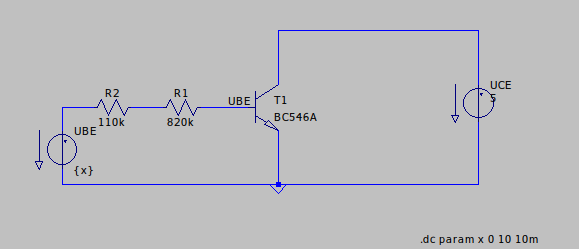
\includegraphics[scale=0.5]{../assets/images/EL1P3/Schaltplan1.png}
  \caption{Schaltplan zur Messung der Kennlinienfelder}
  \label{fig:schalt1}
\end{figure}

\subsection{Ausgangskennlinie}
\label{sec:ausgangskennlinie}

\subsubsection{Vorbereitung}


Wir wollen zunächst das Ausgangskennlinienfeld des Transistors bestimmen. Dazu messen wir $I_{C} = 0...2mA$ und $U_{CE} = 0...10V$ für mindestens 5 verschiedene Basisströme und tragen diese
in LTSpice ab. Für die Basisströme benutzen wir eine variable Spannungsquelle mit einem hochohmigen Vorwiderstand aus der E24-Reihe. Wir wissen aus dem Datenblatt des BC546A, dass die Stromverstärkung bei ca. $B=200$ liegt, wir rechnen also:
\begin{equation}
  \label{eq:1}
  I_{B} = \frac{I_{CE}}{B} = \frac{2mA}{200} = 10\mu A.
\end{equation}
Wir wählen nun eine Spannungsquelle mit einem Maximum von 10V. Um das Maximum von $I_{B} = 10\mu A$ zu bekommen, wollen wir nun den Vorwiderstand unter Berücksichtigung von $U_{BE} = 0,7V$ bestimmen:
\begin{equation}
  \label{eq:2}
  R_{V} = \frac{U_{0}-U_{BE}}{I_{B}} = \frac{10V-0,7V}{10\mu A} = 930k\Omega.
\end{equation}



\subsubsection{Durchführung}
Wir setzen den Wert von $R_{V} = 930k\Omega$ aus den Widerständen $R_{V1} = 110k\Omega$ und $R_{V2} = 820k\Omega$ zusammen (siehe (\ref{fig:schalt1})). Wir variieren nun mit DC-Sweep den Wert von $UCE$ zwischen $0V-10V$ in einem linearen Inkrement von $\Delta I = 10\mu A$. Den Basisstrom nehmen wir für die Werte 2V, 4V, 5V, 6V, 8V und 10V auf und stellen den in einem Kennlinienfeld dar.

\begin{figure}[h]
  \centering
  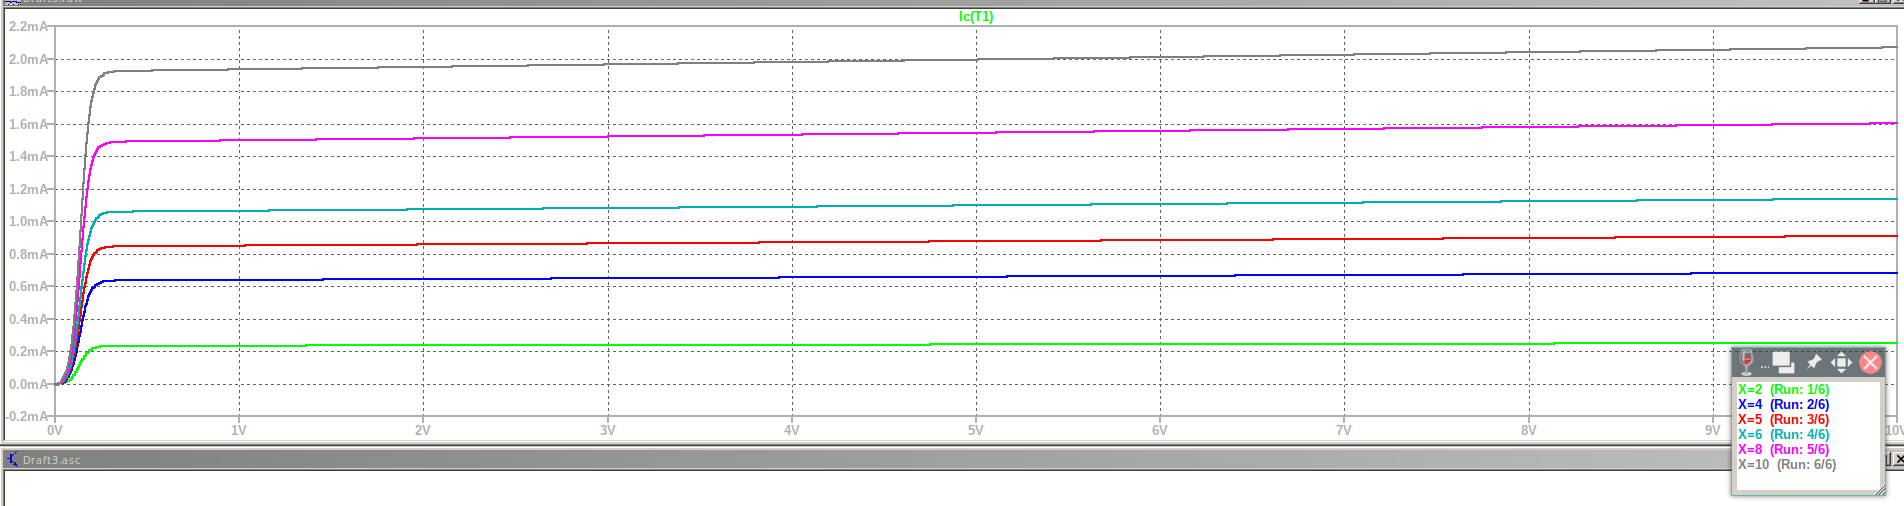
\includegraphics[width=\textwidth]{../assets/images/EL1P3/ausgangskennlinie.png}
  \caption{Ausgangskennlinie der Messschaltung mit verschiedenen Basisströmen}
  \label{fig:ausgang}
\end{figure}

\subsubsection{Auswertung}

Wir lesen nun aus der Abbildung (\ref{fig:ausgang}) den Wert von $I_{C} = 2mA$ an der Stelle $U_{CE} = 5V$ und einem Basisstrom $I_{B} = 10\mu A$. Aus
\begin{equation}
  \label{eq:3}
  B = \frac{I_{C}}{I_{B}} = \frac{2mA}{10\mu A} = 200.
\end{equation}

folgt, dass unsere ermittelte Stromverstärkung der erwarteten Stromverstärkung aus dem Datenblatt bzw. der Vorbereitung entspricht. Um nun die Early-Spannung zu ermitteln, nutzen wir die Cursorfunktion von LTSpice und legen ein Steigungsdreieck an eine der Kennlinien an (wir haben uns für $I_{B} = 2\mu A$ entschieden). Zwischen $U_{CE} = 1V...2V$ ist eine Steigung von $m = 1,818\cdot 10^{-6}$ festzustellen. Von $f_{I_{B1}}(U_{CE}) = f_{2\mu A}(1V) = 233,1964\mu A$ ausgehend bestimmen wir nun den Schnittpunkt der angelegten Geraden mit der X-Achse im Negativen:
\begin{equation}
  \label{eq:4}
  0 = 1,818\cdot 10^{-6}\cdot x + 231,3784\mu A
\end{equation}
Nach dem wir nun die Gleichung nach $x$ auflösen, erhalten wir den Wert $x = -127,27$. Dies ist der Wert der Early-Spannung $U_{A} = -127,27V$.
\newpage

\subsection{Übertragungskennlinie}
\label{sec:ubertr}

Als nächstes wollen wir das Übertragungskennliniefeld des Transistors messen. Wir halten nun die Spannungs $U_{CE} = 5V$ fest und variieren nur noch den Basisstrom zwischen $I_{B} = 0...10\mu A$. Dabei bleibt die Messchaltung beinahe identisch.

\begin{figure}[h]
  \centering
  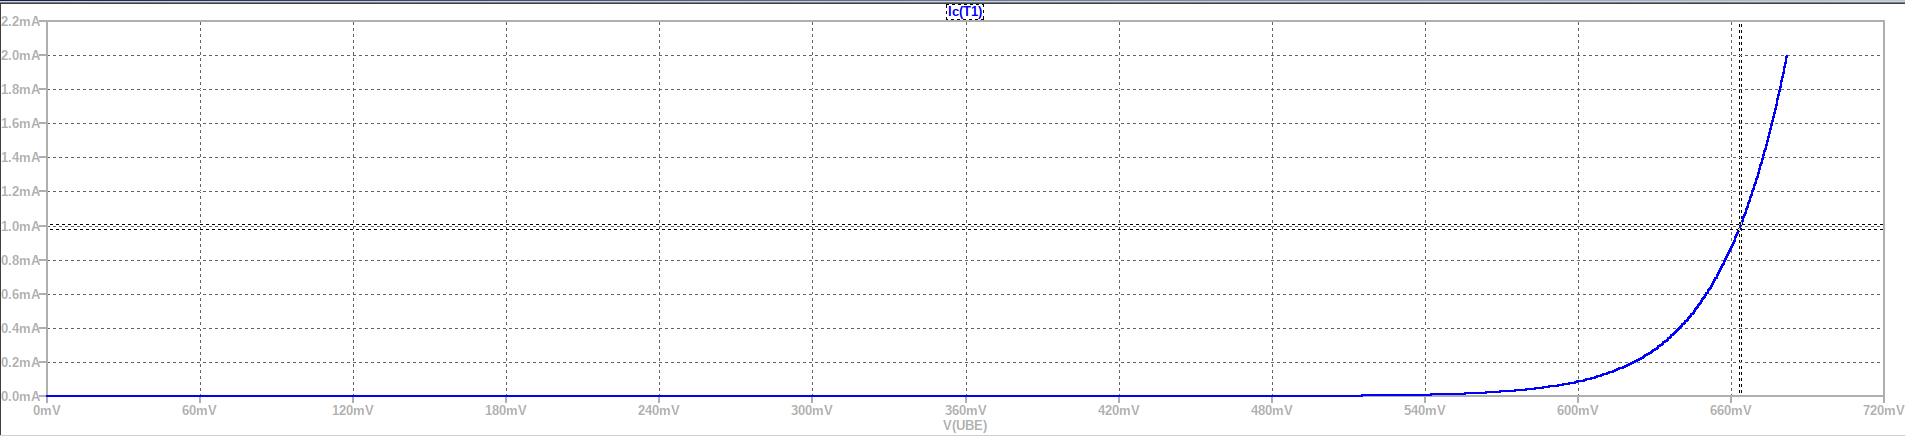
\includegraphics[width=\textwidth]{../assets/images/EL1P3/uebertragungskennlinie.png}
  \caption{Übertragungskennlinienfeld der Messchaltung}
  \label{fig:uebertragungskennlinie}
\end{figure}

\subsubsection{Auswertung}

Wir wollen nun die Steilheit an dem Punkt $I_{C} = 1mA$ bestimmen. Dazu legen wir mit der Cursorfunktion von LTSpice an den Punkt ein Steigungsdreieck an und lesen den gegebenen Wert ab. Es ergibt sich ein Wert von $m = 0,0383771$.

\newpage

\subsection{Steuerkennlinie}

\label{sec:steuerkennlinie}

Zum Schluss wollen wir nun auch die Steuerkennlinie betrachten. Dazu nutzen wir erneut die gleiche Schaltung wie in den letzten beiden Messungen, wobei wir nun $I_{B}$ gegen $I_{C}$ abtragen. Auch hier halten wir $U_{CE} = 5V$ fest, während $I_{B} = 0...10\mu A$ variiert. Das Ergebnis halten wir in einem Plot fest, der eine beinahe lineare Auslenkung besitzt.

\begin{figure}[h]
  \centering
  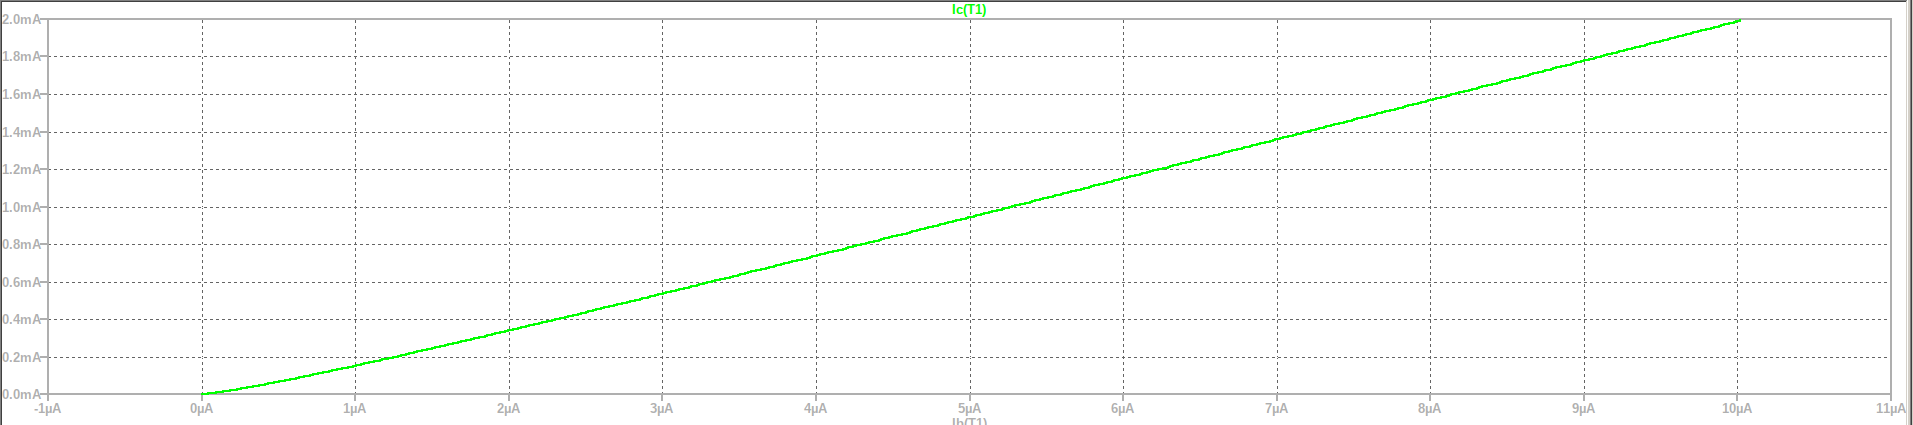
\includegraphics[width=\textwidth]{../assets/images/EL1P3/steuerkennlinie.png}
  \caption{Steuerkennlinie des Messschaltung}
  \label{fig:steuer}
\end{figure}
\newpage
\section{Verstärker in Emitterschaltung}

\begin{task}
  TIn dieser Aufgabe wollen wir eine Verstärkerschaltung mithilfe des vorher analysiertem BC546A simulieren und bestimmte Vorgänge innerhalb der Schaltung genauer untersuchen.
\end{task}

\begin{figure}[h]
  \centering
  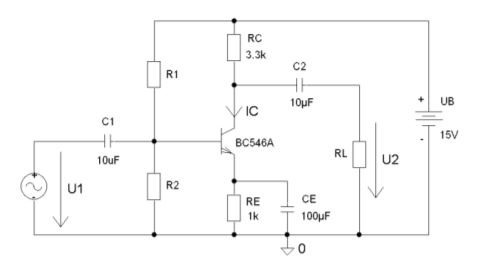
\includegraphics{../assets/images/EL1P3/aufbau aufgabe2.jpg}
  \caption{Versuchsaufbau}
  \label{fig:schalt2}
\end{figure}


\subsection{Arbeitspunkteinstellung}
Für die Arbeitspunkteinstellung wird nur die Gleichspannungsquelle $U_B$ betrachtet und die jeweiligen Maschen ohne Kondensatoren, da diese sich beim Gleichstrom wie unendliche große Widerstände verhalten.
Der Kollektorstrom $I_{C0}$ beträgt 2mA.

\begin{align*}
  &I_B = 10\mu A\\  
  &I_{R1}=10\cdot I_B = 100\mu A\\
  &I_{R2}= 9\cdot I_B = 90\mu A\\
  &U_{R2} = U_{CE} + U_{RE} = 0,7V + (2mA\cdot 1k\Omega) = 2,7V\\
  &R_{2} = \frac{2,7V}{90\mu A} = 30k\Omega\\
  &U_{R1} = U_B - U_{R2} = 15V - 2,7V = 12,3V\\
  &R_{1} = \frac{12,3V}{100\mu A}=123k\Omega
\end{align*}

Da Widerstände aus der E24-Reihe verwendet werden sollen, wird für $R_1$ 120k eingesetzt. \\
Die berechneten Werte werden mithilfe von Simulationen in LTSpice überprüft. Es finden sich die berechneten Werte mit minimalen Abweichungen wieder.

\newpage
\subsection{Wechselspannungsverstärkung}

\begin{figure}[h]
  \centering
  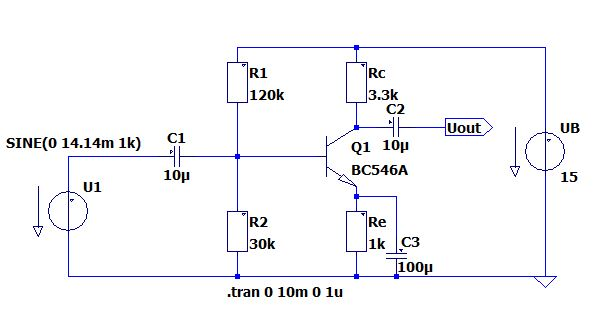
\includegraphics{../assets/images/EL1P3/aufbau 2 2.JPG}
  \caption{Aufbau in LTSpice}
\end{figure}

\begin{figure}[h]
  \centering
  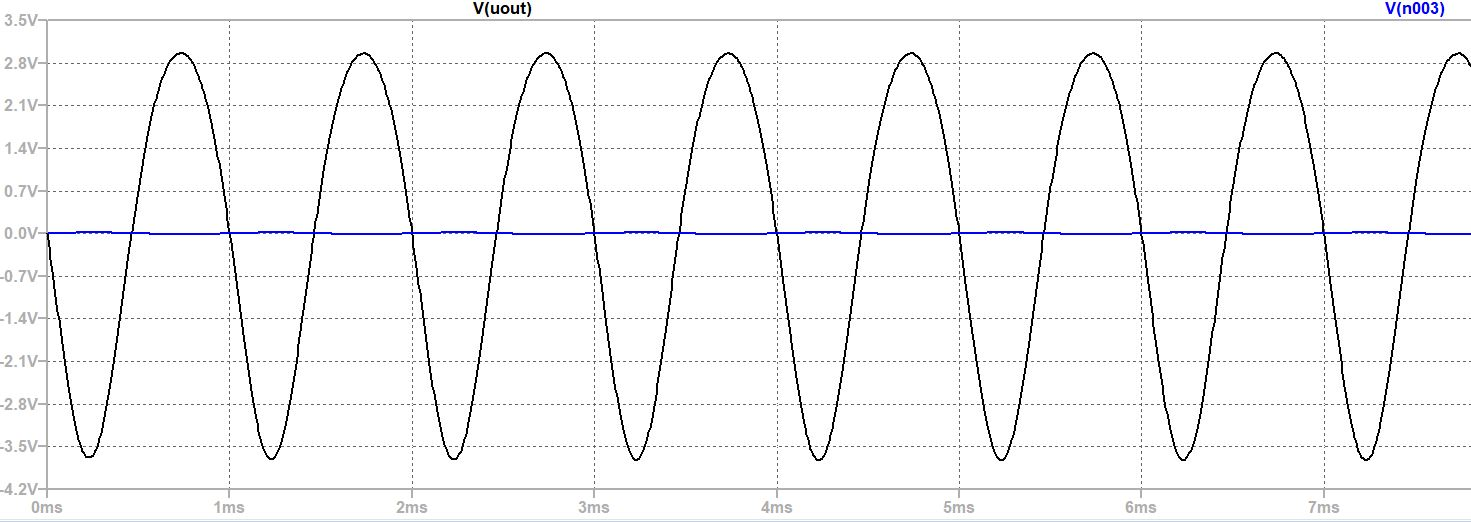
\includegraphics[scale=0.5]{../assets/images/EL1P3/leerlauf aufgabe 2.JPG}
  \caption{Zeitlicher Verlauf der Leerlaufspannung und Eingangsspannung}
\end{figure}


Die Leerlaufspannungsverstärkung beträgt $\frac{U_{out}}{U_{in}}=\frac{2,9V}{14,14mV} =190 $

\subsection{Bestimmung des Ein- und Ausgangswiderstandes (Messung)}

Zur Bestimmung des differentiellen Ausgangswiderstand wird ein Lastwidestand so dimensioniert, dass über ihn genau die Hälfte der Leerlaufspannung abfällt.
\\ Dies ist ungefähr der Fall bei $R_L = 3k\Omega$\\
Nun wird das selbe Verfahren für den differentiellen Eingangswiderstand angewendet, dabei wird ein Widerstand direkt an die Quelle U1 in Reihe mit dem Kondensator C1 geschaltet. 
\\ Hierbei ergibt sich die Hälfte der Leerlaufspannung bei $R = 2,5k\Omega$


\subsection{Bestimmung des Ein- und Ausgangswiderstandes (Näherungsformel)}
\label{sec:bestimmung-des-ein}

Wir wollen nun den differentiellen Ein- und Ausgangswiderstand über die Kennlinienfelder berechnen. Dazu betrachten wir nun zuerst den Eingangskennlinienfeld und legen im Arbeitspunkt $I_{B} = 10\mu A$ ein Steigungsdreieck an, um den differentiellen Eingangswiderstand zu berechnen.
\begin{equation*}
  r_{Id} = \frac{\Delta U_{BE}}{\Delta I_{B}} = \frac{681,86mV - 680,66mV}{10\mu A - 9,5\mu A} = \frac{1,2mV}{0,5\mu A} = 2400\Omega
\end{equation*}
Dieser Wert ist sehr nah an dem Eingangswiderstand, den wir aus der Messung bereits kennen.

Mit dem gleichen Vorgehen wollen wir uns nun auch mit dem Ausgangswiderstand beschäftigen. Dazu betrachten wir nun das Ausgangskennlinienfeld aus der ersten Aufgabe erneut für den Arbeitspunkt $I_{B} = 10\mu A$.

\begin{equation*}
  r_{Od} = \frac{\Delta U_{CE}}{\Delta I_{CE}} = \frac{10V - 5V}{2,069mA - 1,993mA} = \frac{5V}{75,396\mu A} = 66,316k\Omega
\end{equation*}

Wir erkennen, dass aus der differentielle Ausgangswiderstand sehr weit weg von dem in der vorherigen Aufgabe ermitteltem Ausgangswiderstand ist. Woran dies liegt, können wir uns nicht erklären.
\newpage

\section{Spannungsstabilisierung}

\begin{task}
  TBei diesem Versuch werden zwei Schaltung hinsichtlich ihrer Spannungsstabilisierung untersucht bei variierenden Lastwiderständen 
\end{task}

\begin{figure}[h]
  \centering
  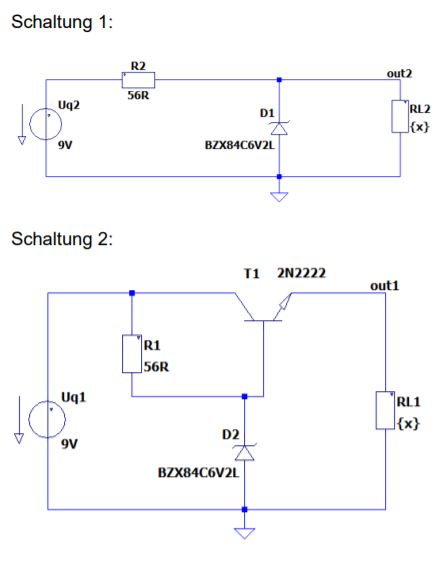
\includegraphics[scale=0.8]{../assets/images/EL1P3/schaltung 3.JPG}
  \caption{Versuchsaufbau}
\end{figure}

\subsection{$U_{out} = f (R_L)$}
\begin{figure}[h]
  \centering
  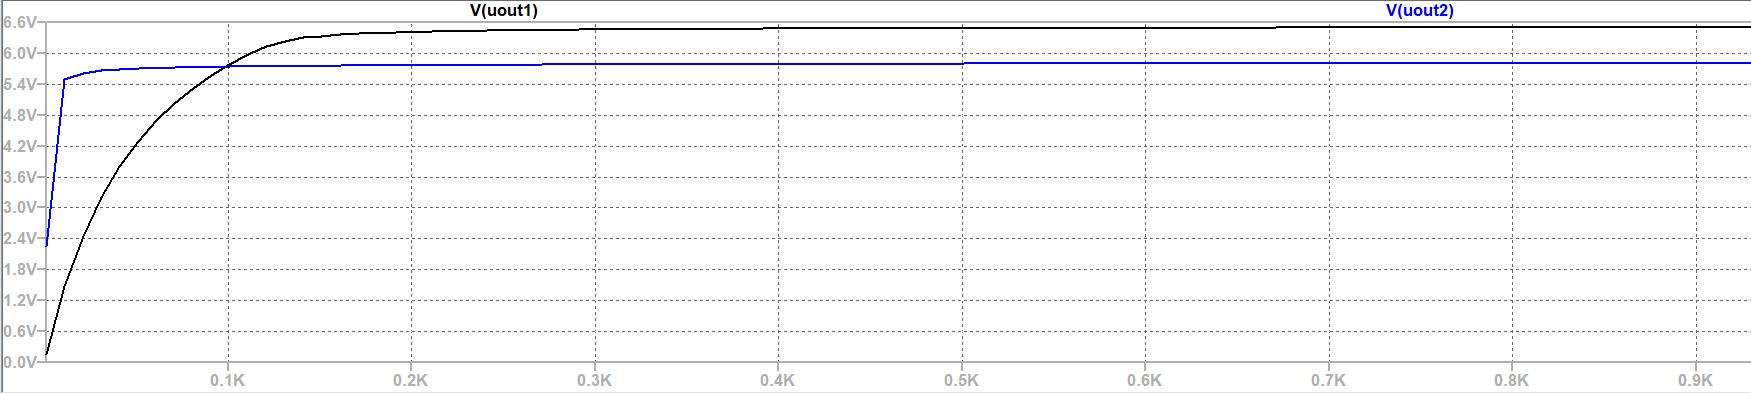
\includegraphics[scale=0.4]{../assets/images/EL1P3/aufgabe 3 u messung.JPG}
  \caption{Stabilisierte Spannungen der beiden Schaltungen}
\end{figure}

\subsection{Auswertung}
Die zeitlichen Verläufe zeigen, dass bei der zweiten Schaltung die Stabilisierung schneller einsetzt, als bei der ersten. Bei kleiner werdenden Lasten ($ca. <100\Omega$) fällt die Spannung der ersten Schaltung exponentiell ab.
Die Spannung der zweiten Schaltung mit Transistor hingegen, hält ab ca. $20\Omega$ ziemlich konstant seine Spannung.
Allerdings ist diese immer um mindestens 0,7V niedriger, da ein Teil der Spannung über den Transistor abfällt.\\
Bei beiden Schaltungen wird die Kennlinie einer Zener-Diode erkennbar. Daher sind Z-Dioden zur Spannungsstabilisierung (geringe Spannungsänderung bei großen Stromänderungen, eindeutige I(U)-Kennlinie) und zur Spannungsbegrenzung geeignet.

\end{document}
